\documentclass{article}



% Language setting

% Replace `english' with e.g. `spanish' to change the document language

\usepackage[english]{babel}



% Set page size and margins

% Replace `letterpaper' with `a4paper' for UK/EU standard size

\usepackage[letterpaper,top=2cm,bottom=2cm,left=3cm,right=3cm,marginparwidth=1.75cm]{geometry}



% Useful packages

\usepackage{amsmath}

\usepackage{amssymb}

\usepackage{graphicx}

\usepackage[colorlinks=true, allcolors=black]{hyperref}

\usepackage{titlesec}
\usepackage{xparse}

\NewDocumentCommand{\qcq}{m o o m}{%
	\ensuremath{\forall #1 \IfValueT{#2}{, #2} \IfValueT{#3}{, #3}  \in  \mathbb{#4}}%
}
\NewDocumentCommand{\ext}{m o o m}{%
	\ensuremath{\exists #1 \IfValueT{#2}{, #2} \IfValueT{#3}{, #3}  \in  \mathbb{#4}}%
}



\title{\textbf{Mathématiques}}

\author{\textbf{Yassin Akkab}}










\graphicspath{ {./Screenshots/} }




\begin{document}
	
	\maketitle
	
	
	
	\tableofcontents
	
	\newpage
	
	
	
	\section{Assertions}
	
	\subsection{Définition }
		
		On appelle assertion (ou proposition) une phrase qui est soit vraie soit fausse (et pas les deux). \\		
		Une assertion peut dépendre d’une variable x, et on la note alors A(x).		
		On dit que deux assertions A et B son équivalentes, ce que l'on note A $\equiv$ B, si elles ont toujours la meme valeur de vérité 
	\subsection{Exemple}
	
	\begin{itemize}
		
		\item {1 \textless 2 est une vraie assertion}
	
		\item { 1 \textgreater 2 est une fausse assertion}
		
		\item {L'assertion A(x) : " x un nombre pair avec x $\in$ $\mathbb{N}$ " dépends de la valeur du x: C'est une assertion vraie si x=0,2,4,6,...,2k et fausse si x=1,3,5,...,2k+1 avec k $\in$ $\mathbb{N}$.
	}
		
		
	\end{itemize}
	
	\subsection{Définition}
	
	Si A et B sont deux assertions, on définit les assertions suivantes :
	
	\begin{enumerate}
		
		\item (non A) : qui est vraie si A est fausse, et fausse sinon, qu’on appelle la négation, notée $\neg$ A
		
		\item (A ou B) : qui est vraie si l’une des deux assertions est vraie, et fausse sinon, qu’on appelle la disjonction, notée A $\cup$ B
		
		\item (A et B) : qui est vraie si les deux assertions sont vraies, et fausse sinon, qu’on appelle la conjonction,
		
		notée A $\cap$ B.
		
	\end{enumerate}
	
	\subsection{Exemple}
		Si A =" n est un multiple de $2^{n}$ " et B =" n est un multiple de $3^{n}$ ", alors :
		\begin{enumerate}
			\item (non A)=“n est impair”
			\item (A ou B)=“n est divisible soit par 2, soit par 3”
			\item (A et B)=“n est un multiple de 6” (par théorème de Gauss)
		\end{enumerate}
	\subsection{Définition}
	
	On appelle table de vérité d’une assertion le tableau donnant sa valeur de vérité en fonction de celles des assertions utilisées pour la construire.
	
	\subsection{Exemple}
	
	La négation, la disjonction et la conjonction ont pour tables de vérité :
	
	
	\begin{center}
		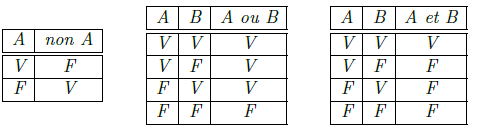
\includegraphics{table1}
	\end{center}
	
	
	
	
	
	
	\newpage
	\subsection{propriété}
	
	
	
	Si A,B,C sont des assertions, on a les propriétés suivantes :
	
	\begin{enumerate}
		
		\item {non(non A) $\equiv$ A}
		
		\item{(A et B) et C  $\equiv$  A et (B et C) }
		
		\item {(A ou B) ou C  $\equiv$  A ou (B ou C)}
		
		\item {A et (B ou C)  $\equiv$  (A et B) ou (A et C)}
		
		\item{ A ou (B et C)  $\equiv$  (A ou B) et (A ou C)}
		
		\item {non (A et B)  $\equiv$  [(non A) ou (non B)]}
		
		\item {non (A ou B)  $\equiv$  [(non A) et (non B)]}
		
	\end{enumerate}
	
	Démonstration :                          
	
	Par exemple, montrons la dernière. On procède par table de vérité :
	
\begin{center}
		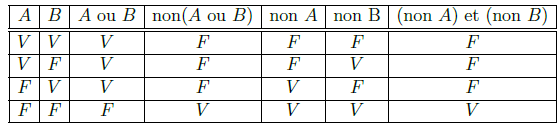
\includegraphics{table2}
\end{center}

\subsection{Exo}
Soient les quatre assertions suivantes :
	
	\begin{enumerate}
		
		\item \ext{x}{R} \qcq{y}{R} x+y $\textgreater$ 0
		\item \qcq{x}{R} \ext{y}{R} x+y $\textgreater$ 0
		\item \qcq{x}{R} \qcq{y}{R} x+y $\textgreater$ 0
		\item \ext{x}{R} \qcq{y}{R} $y^{2}$ $\textgreater$ x  $\textgreater$ 0
	\end{enumerate}
1-Les assertions 1,2,3,4 sont-elles vraies ou fausses? 
\\
\\
2-Donnez leur négation.
	\newpage
	\section{Quantificateurs}
	
	\subsection{Définition}
	
	Soit A(x) une assertion dépendant de x, qui décrit un ensemble E :
	
	\begin{enumerate}
		
		\item {Si, lorsque x décrit E, A(x) est toujours vraie, on écrit : \newline
			
			\begin{center}
				
				$\forall$ x $\in$ $\mathbb{E}$, A(x)  \newline
				
			\end{center}
			
			qu’on lit \textbf{“quel que soit x appartenant à E, A(x)”}. C’est le quantificateur universel.
			
		}
		
		\item {S’il existe x dans E tel que A(x) est vraie, on écrit : \\
			
			\begin{center}
				
				$\exists$ x $\in$ $\mathbb{E}$, A(x)  \newline
				
			\end{center}
			
			qu’on lit\textbf{ “il existe x appartenant à E tel que A(x)”}. C’est le quantificateur existentiel.}
		
	\end{enumerate}
	
	\subsection{Propriété}
	
	Avec les mêmes notations, on a :
	
	
	\begin{enumerate}
		
		\item {non($\forall$ x $\in$ $\mathbb{E}$, A(X)) $\equiv$ $\exists$x $\in$ $\mathbb{E}$, (non A(x))}
		
		\item {non($\exists$ x $\in$ $\mathbb{E}$, A(X)) $\equiv$ $\forall$x $\in$ $\mathbb{E}$, (non A(x))}
		
	\end{enumerate}
	
	\subsection{Remarques}
	
	
	
	\begin{enumerate}
		
		\item {S’il existe un unique x pour lequel A(x) est vrai, on écrit : $\nexists$ x $\in$ $\mathbb{E}$}, A(x).
		
		\item {L’ordre des quantificateurs est importante. Par exemple les assertions : \newline
			
			\begin{center}
				
				[ \qcq{x}{E} , \ext{y}{E}, A(x,y) ] et [ \ext{y}{E} , \qcq{x}{E}, A(x,y) ]
				
			\end{center}
			
			ne sont pas les mêmes : dans la première, y dépend de x ; dans la seconde, y est indépendant de x.
			
		}
		
	\end{enumerate}
	
	\subsection{Exemples}
	
	\begin{enumerate}
		
		\item {L’assertion : \\
			
			\begin{center}
				
				\qcq{n}{N}, \ext{m}{N}, n $\textless$ m
				
			\end{center}
			
			veut dire que : pour tout entier naturel n, il existe un entier naturel m tel que n < m. Elle est
			
			vraie : pour n fixé, l’entier m = n + 1 convient.
			
		}
		
		\item {L’assertion : \\
			
			\begin{center}
				
				\ext{n}{N}, \qcq{m}{N}, n $\textless$ m
				
			\end{center}
			
			veut dire que : il existe un entier naturel m tel que, pour tout entier naturel m, n < m. Elle est
			
			fausse : si n = m par exemple, on ne pourra avoir n $\textless$ m.
			
		}
		
	\end{enumerate}
	
	\subsection{Exo}
	1-Soient les quatre assertions suivantes :
	\begin{enumerate}
		\item \ext{x}{R} \qcq{y}{R} x+y $\textgreater$ 0
		\item \qcq{x}{R} \ext{y}{R} x+y $\textgreater$ 0
		\item \qcq{x}{R} \qcq{y}{R} x+y $\textgreater$ 0
		\item \ext{x}{R} \qcq{y}{R} $y^{2}$ $\textgreater$ x  $\textgreater$ 0
	\end{enumerate}
	a-Les assertions 1,2,3,4 sont-elles vraies ou fausses? 
	\\
	\\
	b-Donnez leur négation.
	\\
	\\
	2-Montrez que : 
	\begin{enumerate}
			\item \qcq{A}[B]{P[E]} A $\cup$ B = A $\cap$ B $\Rightarrow$
			 A=B
			\item \qcq{A}[B][C]{P[E]} A $\cup$ B = A $\cup$ C et A $\cap$ B = A $\cap$ C $\Rightarrow$ B=C 
	\end{enumerate}
	
	\section{Implications, réciproques, contraposées et équivalences}
	\subsection{Définition} Soient A,B sont deux assertions.
	\begin{enumerate}
		\item Si, dès que A est vraie, alors B est aussi vraie : on dit que A implique B, que l’on note \textbf{A $\Rightarrow$ B} \\
		 “ si A alors B ”; on dit alors que : A est une condition suffisante pour
		B, ou que B est une condition nécessaire pour A.
		\item si A implique B et que B implique A : on dit que A est équivalent à B, que l’on note \textbf{A $\Leftrightarrow$ B } \\
		et que l’on lit “A si et seulement si B”; on dit alors que : A est une condition nécessaire et suffisante pour B.
	\end{enumerate}
	Les tables de vérités correspondantes sont :
		\begin{center}
				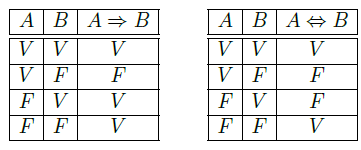
\includegraphics{table3}
		\end{center}
	
	
	
	
	
	
	
	
	
	
	
	
	
	
	
	
	
	
	
	
	
	
	
	
	
	
	
	
	
	
	
	
	
	
	
	
	
	
	
	
	
	
	
	
	
	
	
	
	
	
	
	
	
	
	
\end{document}